\documentclass{article}
\usepackage{bigstrut}
\usepackage{adjustbox}
\usepackage{graphicx}^^M
\graphicspath{ {images/} }
\usepackage[T1]{fontenc}
\usepackage{float}

\usepackage[english]{babel}
\usepackage[utf8]{inputenc}
\usepackage{indentfirst}

\addtolength{\oddsidemargin}{-.875in}
\addtolength{\evensidemargin}{-.875in}
\addtolength{\textwidth}{1.75in}
\addtolength{\textheight}{1in}

\usepackage{hyperref}
\hypersetup{
    colorlinks=true,
    linkcolor=blue,
    filecolor=magenta,      
    urlcolor=cyan,
}

%-----ADDING FIGURES------
%\begin{figure}[h]
%\begin{center}
%\includegraphics[width=\textwidth]{IMAGE_NAME_HERE}
%\caption{CAPTION_HERE}
%\end{center}
%\end{figure}

%-----ADDING TABLES-------
%\begin{table}[h]
%\begin{center}
%\begin{tabular}{c|c|c|c|c}
%& Butterworth & Chebyshev & Linkwitz-Riley & Bessel\\
%\hline
%Passband Accuracy & 10 & 4 & 6 & 9\\
%\hline
%Filter Slope & 7 & 10 & 5 & 6\\
%\hline
%Impulse Response & 5 & 7 & 10 & 3\\
%\hline
%Popularity in Crossover Filters & 3 & 3 & 7 & 3\\
%\hline
%Total & 25 & 24 & 28 & 21\\
%\hline
%Rank & 2 & 3 & 1 & 4\\
%\end{tabular}
%\caption{ADD CAPTION HERE}
%\end{center}
%\end{table}

%-----ADDING IMAGES-----
%\begin{center}
%\includegraphics[width=400px]{Image_NAME_HERE}
%\end{center}


\begin{document}
\title{Sanside Technology}
\begin{titlepage}
    
\includegraphics[width = 150px]{images/SansideLogo.png}
    \hfill
    \hrule
    \vspace{2cm}
    \centering
	{\scshape\LARGE Sanside Technology SEO Optimization Practices\par}
	\vspace{0.5cm}
	{\scshape Marcin Wisniowski: Product Development Intern \par}
    \vspace{2cm}
    \begin{center}
    
\includegraphics[width = 475px]{images/SEO.png}
    \end{center}
    \vspace{0.5cm}
    {\scshape A document to help understand SEO Optimization and a guide to future resources}
\end{titlepage}

\pagenumbering{roman}
\section{Abstract}
With the modern era of Internet resources at the tip of our finger tips, it is often the harder for users to find the resources they are looking for, be it an informative article or a business that provides a service they need. The Internet has become flooded with everyone wanting to show of their own skills or bring something of interest to show the world, but this also causes an over saturation of resources for people to look through. Search Engines have therefore become necessary tools to sift through all the resources and help properly show relevant information to users when they search on them for resources. This guide will look to explore the optimal way to go about creating a website for search engines to pick up and show to the world. 

\tableofcontents

\newpage
\pagenumbering{arabic}

\section{Resources to Learn}
Across this document I will look to try and explain different parts of search engine optimization, but if my explanations are not the best way for you to approach understanding, then I will put these resources at the very beginning of this document to allow you to read up on different SEO Optimization techniques available to learn.

\begin{itemize}
\item \hyperlink{https://varvy.com/}{Varvy: Test your Website and See What you can Improve on}
\item \hyperlink{https://www.site-analyzer.com}{Site Analyzer to See What to Improve}
\item \hyperlink{https://moz.com/beginners-guide-to-seo}{Moz SEO Tutorial}
\item \hyperlink{http://www.google.com/webmasters/tools/richsnippets}{Testing Rich Snippets}
\item \hyperlink{https://developers.google.com/speed/pagespeed/insights/}{Test and see how you can optimize your Website for Speed}
\item \hyperlink{https://www.hildamateiu.com/docs/search-engine-optimization-starter-guide.pdf}{Search Engine Optimization Starter Guide}
\end{itemize}

\section{How SEO Works}
A search engine in plain terms, a robot that scavenges information and then tries to create a database out of it for you to access. In this case, for the biggest search engines like Google, Baidu, Yahoo, Bing, the databases are enormous and the amount of data is expanding exponentially with the internet. But how does it work? How can a website be found by the internet and therefore put into databases. 

\subsection{Finding a Website}
Most search engines send out their army of bots to look across the web and try to find as much new information to add to their databases as possible. For them, the world is a gigantic maze of HTML, with no CSS across any of the web platform to look at. They come across words, pictures, and links and make use of these resources to understand what your website is about. Here are some important notes to remember:

\begin{itemize}
\item These "crawlers" that look across your website navigate through multiple webpages through the use of links. If your website is not linked to other pages across the internet there will be no way for the crawler to find the website in the first place. Similarly, if your own pages are not linked together, i.e. You have to type out a link to get to that website page, the search engine will not be able to find and therefore store that page in its database. Make sure every page incorporates links across it.
\item A strong way to get your page accessed by a database is to link social media accounts to it. This gives the search engine ways to enter your website from outside to store it in databases.
\item These bots, although sophisticated, have a hard time of understanding exactly what is inside pictures. Therefore, Make sure main navigation is done through text and not through clicking images. There are ways to add text to images specifically for bots to understand what they are clicking that will be described later.
\end{itemize}

\subsection{Keywords}
Keywords are basically the search query for people looking for a specific item. When people search for terms, the search engine looks across your website to see if it has to do with those search terms typed it. It checks if the website is relevant and a good result to give back to the user. These are one of the most important to keep in mind when creating a website so we will touch on these later. 

\section{Title Tag}
The title tag on a website is one of the most important parts of each webpage to a search engine. Included in the <head> tag, the <title> tag describes what the website page is about in as few words as possible. Developers should look to customize every single page with a relevant and valuable title tag, so that when searched on a search engine, they can appear for users. Title tags are usually the titles that appear in search results as well. 
\section{Meta Description}
The second most important tag on a website for SEO optimization is the meta description tag. This tag goes hand in hand with the <title> tag to try and explain in a very brief way, in more detail what this webpage is about. In the meta description tag, you should put what you would have to explain this page is about if you only had 30 seconds to describe it. Make sure not to make the meta tag too long or the search engine may cut it short. Also, while it is important to put keywords into both the title and meta description tags, the content will also be read by a human, so make sure that it is legible and understandable, not just a giant list of keywords.

\begin{figure}[h]
\centering
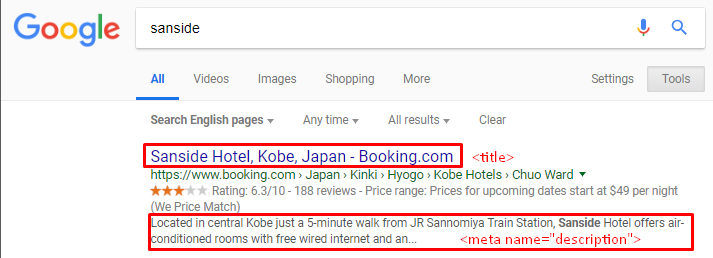
\includegraphics[width=\textwidth]{images/titleandmeta.png}
\caption{Title and Meta Tags appearing in Search Result}
\end{figure}

\section{Header Tags}
Within HTML, a programmer can set different importances of text by putting them within header tags. The search engine then goes through the HTML document and checks for levels of importance. If keywords are found within header tags, they are assumed more important than if the keywords are found within, say, a paragraph tag or a lower header tag. 

\section{Images}
Search Engines are unable to see what images look like, and therefore the programmer should put a few extra lines of codes to help explain what the pictures are showing. <image alt=""> tags are used to help explain what the pictures are about. While almost no one will see this, it is still important to include for the bots to accurately identify the images.

\section{Deciding on Keywords}
While the actual algorithms for finding keywords are hidden from the users making content, there are a few choices that can help with understanding your users and how they are finding out about you. 
\subsection{Google Trends}
Good Trends is the most upfront way of comparing two different keywords. This allows people to type two different keywords and compare their searches by users to see which is most popular. However, be careful about always choosing the more popular one. It is important to get a wide audience, but it also important to understand the competition you will likely gain by picking a more broad topic.
\hyperlink{http://trends.google.com/trends/explore}{Google Trends Link}

\begin{figure}[h]
\centering
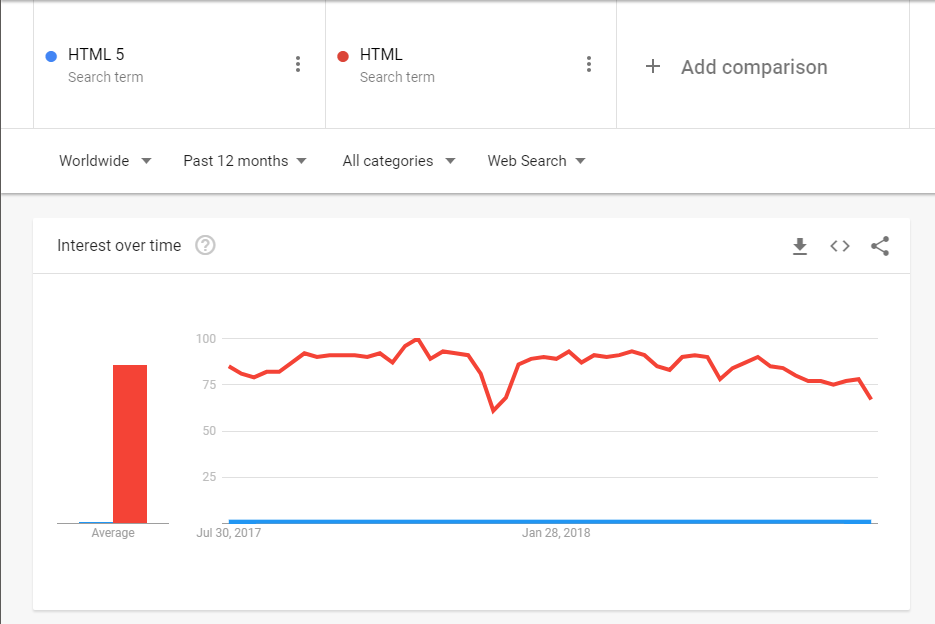
\includegraphics[width=\textwidth]{images/HTML.png}
\caption{The keyword "HTML" is far more popular than "HTML5"}
\end{figure}

\subsection{Autocompletion}
Many search engines are able to help users with their typing keywords by recommending autocomplete phrases. While your company may be focusing on a specific field, if they do not contain popular phrases in that field, they will be much harder to find. People can look to change their content to try and grab the attention of one of these more common keywords and use it more frequently in their page to bring more views and interest to the page.

Similarly, at the bottom of most search engines, the website will give you similar searches that other users have looked for. Use these to further understand what is trendy and what is being search for to optimize what to write about.

\section{Rich Snippets}
Rich Snippets are little boxes of content that appear before going into the website itself. For example, when searching for a company, the company name, logo, and CEO might appear within the search results before having to go into the page itself. Similarly, if searching for a recipe for food, you can usually find the list of steps inside the search instead of having to click on a website. This makes snippets very successful at drawing people's attention and giving them instant content that they might be searching for. Rich snippets also help people decide if something is relevant before they click on it.

\begin{figure}[h]
\centering
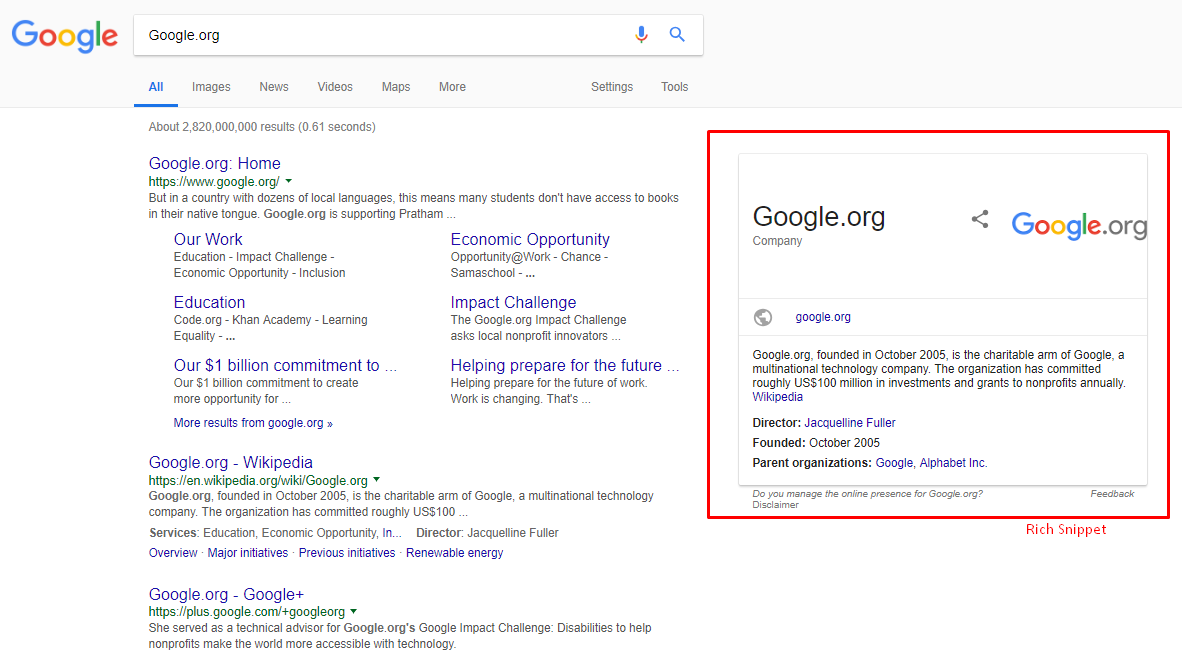
\includegraphics[width=400px]{images/richsnippet.png}
\caption{Rich Snippet Showing information about the company Google}
\end{figure}


Snippets can also help enhance a users' experience by giving relevant information or easier access to things that they might be searching. Rich snippets have been successfully used to give users information but also to do actions, including sign up for events or watch videos and listen to music. Very often, rich snippets increase the chance someone will click on your page's results and can make users feel more trustworthy of your company. Many companies see 20-30\% more clicks when using rich snippets

\hyperlink{www.schema.org}{Schema.org} is a website formed by Google, Bing, and Yahoo, the biggest US search engines to try and make a standard for microdata that is used for rich snippets. You can learn more by going to schema.org or reading the resources found at the beginning of the document.

\begin{figure}[h]
\centering
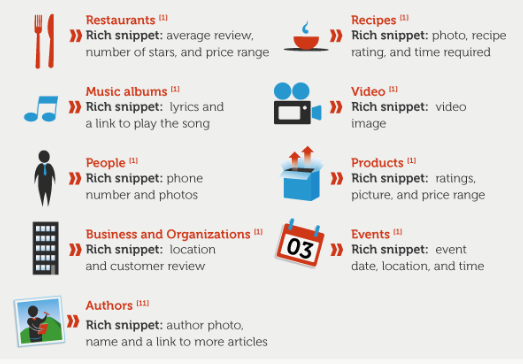
\includegraphics[width=400px]{images/snippet2.png}
\caption{Rich Snippet Possibilities}
\end{figure}

\section{Getting Recognized}
\subsection{Social Media}
Since the search engine looks for ways to enter your site, social media is a great resource for getting your website distributed and recognized. When creating social media accounts make sure to put the website itself onto the profiles of the social media accounts in order to have more ways of entering your site. 

Similarly, you can use social media in order to promote different parts of your website and try to find an audience that enjoys what you are doing or are interested in what you are doing. The most important part of getting noticed and growing big is having something that you are interested in sharing, and making it interesting and engaging for your audience; something that they also would like to further share.

\subsection{Blogs/News}
If you have anything interesting to share or have created something new, one of the best ways to get some promotion for your company and products is to reach out to relevant reviews or blogs or news outlets and try to make them become interested in your product. However, make sure that you ask relevant promoters, because you do not want people that are interesting in clothes to come to a mobile gaming site. Still, you are losing nothing by trying to send out emails to some blogs, or reviewers and getting them to write about your product. Just make sure it is a good product!

\end{document}